% !TeX root = ../main.tex

% Edit this title for each week's entry.
\section{Week 9 - Taxation}

\topic{Corporate Taxation}

\heading{What Are Corporate Taxes?}
\begin{itemize}
    \item In your personal life, you pay income taxes on the money you earn (minus some deductions)
    \item Corporations pay \rb{corporate taxes} on their \dbb{profits}
\end{itemize}

\heading{Project Cash-flows Before Tax}
\begin{center}
    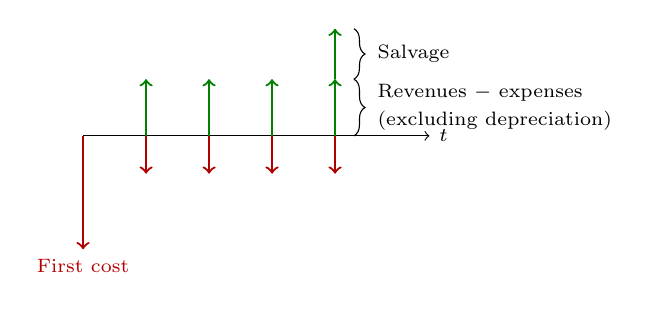
\begin{tikzpicture}[scale=0.8]
        \draw[->] (0,0) -- (5.5,0) node[right] {\scriptsize $t$};
        \draw[->,thick,red!70!black] (0,0) -- (0,-1.8) node[below] {\scriptsize First cost};
        \foreach \x in {1,...,4}{
            \draw[->,thick,green!50!black] (\x,0) -- (\x,0.9);
            \draw[->,thick,red!70!black] (\x,0) -- (\x,-0.6);
        }
        \draw[->,thick,green!50!black] (4,0.9) -- (4,1.7);
        \draw[decorate,decoration={brace,amplitude=4pt}] (4.3,1.7) -- (4.3,0.9) node[midway,right=5pt] {\scriptsize Salvage};
        \draw[decorate,decoration={brace,amplitude=4pt}] (4.3,0.9) -- (4.3,0) node[midway,right=5pt,align=left] {\scriptsize Revenues $-$ expenses\\[-2pt]\scriptsize (excluding depreciation)};
    \end{tikzpicture}
    \\[2pt] \textit{\small Discounted using MARR. Depreciation is not shown (it is not a cash-flow)}
\end{center}

\begin{definition}[Corporate Tax]
    The amount of tax owed depends on profits:
    \[\boxed{\begin{gathered}
        \text{Taxable income} = \text{Revenues} - \text{Expenses}\\[2pt]
        \text{Corporate tax} = \text{Taxable income} \times t\\[4pt]
        \begin{array}{@{}l@{}}
            t: \text{(flat) corporate tax rate}
        \end{array}
    \end{gathered}}\]
    \begin{itemize}
        \item Paying tax $\to$ \dbb{negative} cash-flow
        \item Tax savings $\to$ \dbb{positive} cash-flow!
    \end{itemize}
\end{definition}

\begin{example}[From the Income Statement]
    \begin{center}
    \begin{tabular}{lr}
        \toprule
        Revenue & 12,200 \\
        \quad Cost of sales & 6,000 \\
        Gross margin & 6,200 \\
        \quad Selling and admin (SG\&A) & 4,200 \\
        \rb{EBITDA} & 2,000 \\
        \quad Depreciation & 60 \\
        \rb{EBIT} & 1,940 \\
        \quad Interest expense & 30 \\
        Income before taxes & 1,910 \\
        \quad Provision for taxes & 764 \\
        \b{Net income} & \b{1,146} \\
        \quad Dividends & 1,000 \\
        Addition to equity & 146 \\
        \bottomrule
    \end{tabular}
    \end{center}
    \db{Tax is charged on income before taxes, after \dbb{all} expenses (including depreciation and interest) are subtracted: $t = 764/1910 = 40\%$. Dividends come \dbb{after} tax, so they don't reduce it.}
\end{example}

\heading{What Affects Taxable Income}
\begin{center}
\begin{tabular}{p{0.44\linewidth}p{0.44\linewidth}}
    \toprule
    \b{Revenues/gains} (\dbb{increase} tax owed) & \b{Expenses/deductions} (\dbb{decrease} tax owed) \\
    \midrule
    Sales revenues & Cost of goods sold, general expenses \\
    Interest revenues (interest earned) & Interest expenses \\
    Capital gains (asset sold above cost/book value) & Depreciation expenses \\
    & Capital losses (asset sold below book value) \\
    \bottomrule
\end{tabular}
\end{center}
\b{Not} deductible: \dbb{dividends}, \dbb{asset purchases}, and others.

\heading{How Taxation Affects Cash-flows}
\begin{center}
    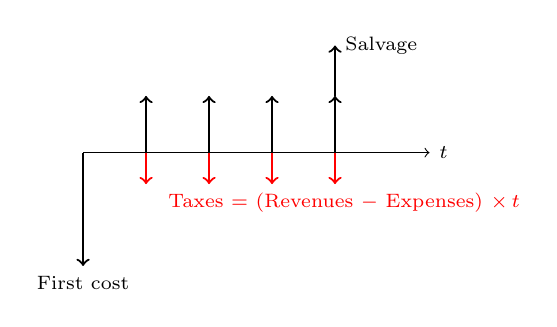
\begin{tikzpicture}[scale=0.8]
        \draw[->] (0,0) -- (5.5,0) node[right] {\scriptsize $t$};
        \draw[->,thick] (0,0) -- (0,-1.8) node[below] {\scriptsize First cost};
        \foreach \x in {1,...,4}{
            \draw[->,thick] (\x,0) -- (\x,0.9);
            \draw[->,thick,red] (\x,0) -- (\x,-0.5);
        }
        \draw[->,thick] (4,0.9) -- (4,1.7) node[right] {\scriptsize Salvage};
        \node[red,right] at (1.2,-0.8) {\scriptsize Taxes $=$ (Revenues $-$ Expenses) $\times\, t$};
    \end{tikzpicture}
\end{center}

\begin{example}[Reflection: Salaries]
    If a company spends \$100,000 on salaries, how does it affect its
    corporate taxes?
    \\\db{Salaries are an \dbb{expense}: taxable income drops by \$100,000, so tax drops by $100{,}000\,t$. The after-tax cost of the salaries is only $100{,}000(1 - t)$ (e.g.\ \$75,000 at $t = 25\%$).}
\end{example}

\begin{example}[Reflection: Equipment]
    If a company spends \$100,000 on equipment, how does it affect its
    corporate taxes?
    \\\db{\dbb{No immediate effect}: buying an asset just swaps cash for equipment on the balance sheet, so it is not an expense. The cost is deducted gradually through depreciation instead.}
\end{example}

\heading{Assets Affect Taxation Through Depreciation}
Purchasing an asset has no immediate effect on corporate taxes. But once the
company holds an asset, it affects taxes in two ways:
\begin{itemize}
    \item Claiming \b{depreciation}
    \item \b{Capital gains/losses} when it is sold
\end{itemize}

\begin{definition}[Effect of Taxation on Rates of Return]
    Discounting after-tax cash-flows requires a lower rate:
    \[\boxed{\text{MARR}_{\text{after tax}} \approx \text{MARR}_{\text{before tax}}(1 - t), \qquad \text{IRR}_{\text{after tax}} \approx \text{IRR}_{\text{before tax}}(1 - t)}\]
\end{definition}

\heading{Summary}
\begin{enumerate}
    \item Corporate taxes depend on taxable income (revenues $-$ expenses) and the tax rate
    \item Revenues $\to$ increase tax; expenses $\to$ decrease tax
    \item Asset purchase $\to$ \b{no immediate} impact on taxes
    \item Taxes reduce MARR and IRR by a factor of about $(1 - t)$
\end{enumerate}

\topic{Capital Cost Allowance (CCA)}

\heading{Depreciation Saves You Taxes!}
\begin{itemize}
    \item Depreciation itself is \b{not} a cash-flow
    \item But claiming depreciation lowers taxable income $\to$ \dbb{tax savings} (a positive cash-flow)
    \item Time value of money: the sooner depreciation is claimed, the more the savings are worth
\end{itemize}

\begin{remark}
    Claiming depreciation earns you money!
\end{remark}

\begin{definition}[Capital Cost Allowance (CCA)]
    The \dbb{Canadian} system for calculating depreciation for tax purposes
    (Canada Revenue Agency). Assets are grouped into \rb{CCA asset classes},
    and each class has a \rb{CCA rate} (depreciation rate).
\end{definition}

\begin{center}
\begin{tabular}{ll}
    \toprule
    Book depreciation term & Tax depreciation term \\
    \midrule
    Depreciation & \rb{Capital cost allowance (CCA)} \\
    Book value & \rb{Undepreciated capital cost (UCC)} \\
    Salvage value & \rb{Proceeds from disposition} \\
    \bottomrule
\end{tabular}
\end{center}

\heading{Important Point 1: Pooling Assets}
\begin{itemize}
    \item All assets in a class are \dbb{pooled} together, and CCA is based on the UCC of \b{all} assets in that class
    \item Assets are \b{not} depreciated individually!
\end{itemize}
\begin{center}
\begin{tabular}{lcc}
    \toprule
    Description & Class & Rate \\
    \midrule
    Bridges, culverts, dams, buildings, wiring, plumbing, HVAC & 1 & 4\% \\
    General property: furniture, fixtures, equipment, tools $>$ \$500 & 8 & 20\% \\
    Autos, trailers, general-purpose computers, terminals, trucks & 10 & 30\% \\
    Most manufacturing and processing equipment & 43 & 30\% \\
    General-purpose IT equipment and systems software & 50 & 55\% \\
    \bottomrule
\end{tabular}
\end{center}

\heading{Important Point 2: Half-Year Rule}
CCA is a slightly modified \b{declining balance} method. Only \dbb{half} of
this year's additions are depreciated in the year they are bought (the
\rb{half-year rule}, established in 1980):
\[\boxed{\begin{gathered}
    \text{CCA}_n = d\left(\frac{\text{Additions}_n}{2} + \text{UCC}_{n-1}\right)\\[2pt]
    \text{UCC}_n = \text{UCC}_{n-1} + \text{Additions}_n - \text{CCA}_n\\[4pt]
    \begin{array}{@{}l@{}}
        d: \text{CCA rate of the class}\\
        \text{Additions}_n: \text{cost of assets added to the class in year } n
    \end{array}
\end{gathered}}\]
\db{Compare plain declining balance: $D = d(\text{Additions} + BV_{\text{last year}})$, $BV = BV_{\text{last year}} + \text{Additions} - D$.}

\begin{example}[CCA for New Purchases]
    Your company purchased \$5000 worth of desks (class 8, CCA rate 20\%).
    What are the CCA and UCC for the first 4 years? (Nothing else is in the
    same CCA pool.)
    \begin{center}
    \begin{tabular}{clr}
        \toprule
        Year & CCA & UCC \\
        \midrule
        1 & $0.2(5000/2 + 0) = 500$ & $5000 - 500 = 4500$ \\
        2 & $0.2(4500) = 900$ & 3600 \\
        3 & $0.2(3600) = 720$ & 2880 \\
        4 & $0.2(2880) = 576$ & 2304 \\
        \bottomrule
    \end{tabular}
    \end{center}
    \db{Year 1 gets only half the usual 20\%. After that it is ordinary declining balance on the UCC.}
\end{example}

\begin{definition}[Tax Savings from Depreciation]
    There is no out-of-pocket expense from depreciation, but claiming it
    saves taxes:
    \[\boxed{\text{Tax savings}_n = \text{CCA}_n \times t}\]
\end{definition}

\heading{CCA Rules on Disposition}
The UCC (book value) can differ from the salvage value $S$ when the asset is
sold. Let $P$ be the original cost of the asset.
\begin{center}
\small
\begin{tabular}{p{0.34\linewidth}p{0.14\linewidth}p{0.42\linewidth}}
    \toprule
    Case & Remove from UCC & Tax implication \\
    \midrule
    \rb{Open books}: other assets remain in the class & $S$ & No taxes now \\
    \midrule
    \rb{Closed books}, case 1: $S < BV$ & $BV$ & Claim \rb{terminal loss} $(BV - S)$ \\
    \rb{Closed books}, case 2: $BV < S < P$ & $BV$ & Report \rb{recapture} $(S - BV)$ \\
    \rb{Closed books}, case 3: $S > P$ & $BV$ & Report recapture $(P - BV)$, plus a \rb{capital gain} $(S - P)$ \\
    \bottomrule
\end{tabular}
\end{center}
\begin{itemize}
    \item \b{Open books}: selling the asset does not close out the pool. The UCC is simply reduced by $S$, and the difference keeps being depreciated with the rest of the pool
    \item \b{Closed books} (no other items in the pool): the pool is settled right away. A terminal loss is deductible (tax \dbb{savings}); recapture is taxable income (tax \dbb{owed})
\end{itemize}

\begin{remark}
    In these notes (as in the Eric's Almonds example below), CCA is still
    claimed for the year of sale, and the asset is then disposed of at the
    end of that year.
\end{remark}

\begin{example}[Open Books]
    Your company purchased \$5000 worth of desks (class 8). In year 5, the
    desks are sold for \$1500. What is the CCA for year 5, and what is the
    gain/loss? \b{There are other assets in class 8.}
    \\\db{From the CCA table above, $\text{UCC}_4 = \$2304$, so this part of the pool contributes}
    \[\text{CCA}_5 = 0.2(2304) = \db{\$460.80}, \qquad \text{UCC} = 2304 - 460.80 = \$1843.20\]
    \db{Selling the desks removes $S = \$1500$ from the pool: $1843.20 - 1500 = \$343.20$ stays in the pool and keeps being depreciated. \dbb{No gain or loss} is reported, so there is no tax effect now.}
\end{example}

\begin{example}[Disposition: Loss]
    Same desks sold for \$1500 in year 5, but \b{no other assets are in
    class 8}.
    \\\db{$\text{CCA}_5 = \$460.80$ and $BV = \$1843.20$ as before. The class closes with $S = 1500 < BV$:}
    \[\text{Terminal loss} = 1843.20 - 1500 = \db{\$343.20}\]
    \db{This is deducted from taxable income, saving $343.20\,t$ in taxes.}
\end{example}

\begin{example}[Disposition: Recapture]
    Same desks sold for \$2500 in year 5, with \b{no other assets in class
    8}.
    \\\db{$\text{CCA}_5 = \$460.80$ and $BV = \$1843.20$. Now $BV < S = 2500 < P = 5000$:}
    \[\text{Recapture} = 2500 - 1843.20 = \db{\$656.80}\]
    \db{Too much CCA was claimed over the years, so this amount is added back to taxable income and taxed: $656.80\,t$ owed.}
\end{example}

\heading{Summary}
\begin{enumerate}
    \item \b{CCA} is the depreciation method for tax purposes: assets are \b{pooled} by class and depreciated as a pool
    \item Declining balance with the \b{half-year rule}
    \item On disposition: open books $\to$ reduce UCC by $S$; closed books $\to$ terminal loss, recapture, or capital gain
    \item Claiming depreciation earns you money!
\end{enumerate}

\topic{Calculating PW with Taxes (Explicit Method)}

\heading{Calculating PW with Taxes}
\begin{enumerate}
    \item \b{MARR}: use the \dbb{after-tax} MARR
    \item \b{Annual revenues}: reduced by taxes, $A(1 - t)$
    \item \b{First cost}: no direct effect
    \item \b{Depreciation}: follow CCA depreciation rules; each year saves $\text{CCA}_n \times t$
    \item \b{Salvage value}: follow CCA disposition rules
\end{enumerate}

\begin{example}[Eric's Almonds]
    Eric's Almonds sells packaged almonds in Canada and is deciding on
    almond packaging machinery:
    \begin{center}
    \begin{tabular}{llr}
        \toprule
        Quantity & Symbol & Value \\
        \midrule
        First cost & $FC$ & \$26,000 \\
        Annual net savings & $A$ & \$10,000 \\
        Salvage value (after 10 years) & $S$ & \$2000 \\
        Life & $N$ & 10 years \\
        After-tax MARR & $i$ & 15\% \\
        Tax rate & $t$ & 25\% \\
        CCA rate (class 8) & $d$ & 0.2 \\
        \bottomrule
    \end{tabular}
    \end{center}
    Eric's Almonds is profitable. What is the after-tax PW of this machine
    if it is their \b{only item in this CCA class}?
    \begin{enumerate}[label = \arabic*.]
        \item \b{MARR}: \db{the after-tax MARR is given, $i = 15\%$. (If only the before-tax MARR were given, use $i_{\text{after tax}} = i_{\text{before tax}}(1 - t)$.)}
        \item \b{Annual revenues} are taxed:
        \[\text{PW}(A) = A(1 - t)(P/A,15\%,10) = 7500(5.0188) = \db{\$37{,}641}\]
        \item \b{First cost}: \db{no tax effect at purchase, $\text{PW}(FC) = -\$26{,}000$.}
        \item \b{Tax savings from depreciation} (half-year rule):
        \begin{center}
        \small
        \begin{tabular}{crrr}
            \toprule
            Year & CCA & UCC & Tax savings ($\times 0.25$) \\
            \midrule
            1 & $0.2(26{,}000/2) = \db{2600}$ & \db{23,400} & \db{650} \\
            2 & $0.2(23{,}400) = \db{4680}$ & \db{18,720} & \db{1170} \\
            3 & 3744 & 14,976 & 936 \\
            4 & 2995 & 11,981 & 749 \\
            5 & 2396 & 9585 & 599 \\
            6 & 1916 & 7668 & 479 \\
            7 & 1534 & 6134 & 383 \\
            8 & 1227 & 4907 & 307 \\
            9 & 981 & 3926 & 245 \\
            10 & 785 & \db{3141} & 196 \\
            \bottomrule
        \end{tabular}
        \end{center}
        \[\text{PW}(TS) = \sum_{n=1}^{10} \text{CCA}_n\, t\,(P/F,15\%,n) = \db{\$3361}\]
        \item \b{Disposition} (closed books): \db{$S = 2000 < \text{UCC}_{10} = 3141$, so it is a \dbb{terminal loss} of $3141 - 2000 = \$1141$, which saves $0.25(1141) = \$285$ in tax. The year-10 disposal cash-flow is}
        \[2000 + 285 = \$2285, \qquad \text{PW}(S) = 2285(P/F,15\%,10) = 2285(0.24718) = \db{\$565}\]
    \end{enumerate}
    \db{Sum all together:}
    \[\text{PW} = -26{,}000 + 37{,}641 + 3361 + 565 = \dbb{\$15{,}567}\]
    \db{$\text{PW} > 0$, so the machine is worth buying.}
\end{example}

\heading{Summary}
Calculate PW including tax implications year by year:
\begin{enumerate}
    \item Taxes on revenues: $A(1 - t)$
    \item Tax savings from depreciation: $\text{CCA}_n \times t$
    \item Gains/losses from asset disposition (terminal loss, recapture, capital gain)
\end{enumerate}

\topic{Calculating PW with Taxes (Tax Benefit Factor)}

\begin{definition}[Tax Benefit Factor ($\tau$)]
    An asset has an inherent value, but also a \dbb{value associated with
    tax benefits}. The tax benefit factor is the present value of all the
    future tax savings per dollar spent on the asset today:
    \[\boxed{\tau = \frac{\text{PW(tax savings)}}{FC}}\]
    E.g.\ $\tau = 0.2$: every dollar spent brings future tax savings with a
    total PW of \$0.20.
\end{definition}

\heading{Tax Benefit Factors}
$\tau$ depends on the depreciation method, the tax rate, and the time value
of money:
\[\boxed{\begin{gathered}
    \tau_{db} = \frac{td}{i + d}, \qquad \tau_{1/2} = \frac{td}{i + d}\left(\frac{1 + i/2}{1 + i}\right)\\[4pt]
    \begin{array}{@{}l@{}}
        i: \text{after-tax MARR}\\
        d: \text{depreciation (CCA) rate}\\
        t: \text{tax rate}
    \end{array}
\end{gathered}}\]
\begin{itemize}
    \item $\tau_{db}$ (\b{declining balance}): applies to asset \dbb{disposition} in the CCA system
    \item $\tau_{1/2}$ (\b{declining balance with half-year rule}): applies to asset \dbb{purchase} in the CCA system
\end{itemize}
\db{Both assume the CCA on the asset continues forever (the UCC never quite reaches 0). The half-year rule delays half of the first-year CCA, so $\tau_{1/2} < \tau_{db}$.}

\begin{example}[Reflection: Higher or Lower $\tau$?]
    From a company's point of view, would you choose a depreciation method
    with a higher or lower tax benefit factor?
    \\\db{\dbb{Higher}: a larger $\tau$ means the tax savings arrive sooner and are worth more today, which lowers the effective cost of the asset.}
\end{example}

\heading{Using the Tax Benefit Factor}
\begin{itemize}
    \item Spending $FC$ on an asset: the \rb{effective first cost} is reduced by the future tax savings:
    \[\boxed{\text{PW}(FC) = -FC + FC\,\tau_{1/2} = -FC\left(1 - \frac{td}{i + d}\left(\frac{1 + i/2}{1 + i}\right)\right)}\]
    \item Selling an asset for $S$ that reduces the asset pool by $R$: the \rb{effective salvage value} is reduced because the future tax savings on $R$ are lost:
    \[\boxed{\text{PW}(S) = (S - R\,\tau_{db})(P/F,i,N) = \left(S - R\,\frac{td}{i + d}\right)(P/F,i,N)}\]
\end{itemize}

\begin{example}[Eric's Almonds Using $\tau$]
    Same machine as before ($FC = \$26{,}000$, $A = \$10{,}000$,
    $S = \$2000$, $N = 10$, $i = 15\%$, $t = 25\%$, $d = 0.2$). What is the
    after-tax PW if the machine is
    \begin{itemize}
        \item[A.] one of many items in this CCA class?
        \item[B.] the only item in the class?
    \end{itemize}
    \db{Compute the effective first cost, the annual after-tax revenues (same as before), and the effective salvage value (depends on the case).}
    \begin{enumerate}[label = \arabic*.]
        \item \b{First cost + tax savings from depreciation}:
        \[\tau_{1/2} = \frac{0.25(0.2)}{0.15 + 0.2}\left(\frac{1.075}{1.15}\right) = 0.13354\]
        \[\text{PW}(FC) = -26{,}000(1 - 0.13354) = \db{-\$22{,}528}\]
        \db{Every dollar spent on the machine effectively costs only \$0.866.}
        \item \b{After-tax revenues}: \db{as before,}
        \[\text{PW}(A) = 10{,}000(1 - 0.25)(P/A,15\%,10) = \db{\$37{,}641}\]
        \item \b{Disposition}, $\tau_{db} = 0.05/0.35 = 0.14286$:
        \begin{itemize}
            \item \b{Case A} (\dbb{open books}): \db{receive $S = 2000$; the pool shrinks by $R = S = 2000$, so the tax savings on that \$2000 are lost; no tax on gain/loss:}
            \[\text{PW}(S) = (2000 - 2000(0.14286))(0.24718) = \db{\$424}\]
            \item \b{Case B} (\dbb{closed books}): \db{receive $S = 2000$; the pool loses the whole remaining UCC, $R = \text{UCC}_{10} = 3141$; and the terminal loss $3141 - 2000 = 1141$ saves $0.25(1141) = \$285$ in tax:}
            \[\text{PW}(S) = (2000 - 3141(0.14286) + 285)(0.24718) = \db{\$454}\]
        \end{itemize}
    \end{enumerate}
    \db{Sum all together:}
    \begin{align*}
        \text{Case A: } \text{PW} &= -22{,}528 + 37{,}641 + 424 = \dbb{\$15{,}537}\\
        \text{Case B: } \text{PW} &= -22{,}528 + 37{,}641 + 454 = \dbb{\$15{,}567}
    \end{align*}
    \db{Case B matches the explicit year-by-year method exactly (\$15,567), as it should. The $\tau$ method is much faster since no CCA table is needed (except for $\text{UCC}_{10}$ in Case B).}
\end{example}

\heading{Summary}
\begin{enumerate}
    \item \b{Tax benefit factor}: the equivalent fraction of an asset purchase that is recovered through future tax savings
    \item The purchase reduces the first cost by a factor of $(1 - \tau_{1/2})$
    \item On disposition, the tax benefits on the amount $R$ removed from the pool are given up: $S - R\,\tau_{db}$
\end{enumerate}
